\section{Esercizio 7 -- Moltiplicatore di Booth}
\subsection{Esercizio 7.1}
L'obiettivo è progettare, implementare e simulare un moltiplicatore di Booth capace di effettuare il prodotto di due stringe A e B, entrambi di 8 bit, restituendo un risultato a 16 bit [Figura \ref{fig:7_1_BOOTH_MULTIPLIER}].

Nell'automa [Figura \ref{fig:booth_multiplier_tb}] è stato omesso il ritorno a zero dei segnali di controllo per semplificare la visualizzazione. È da intendersi che essi vengano azzerati nello stato succesivo alla loro abilitazione.

\begin{figure}[h]
    \centering
    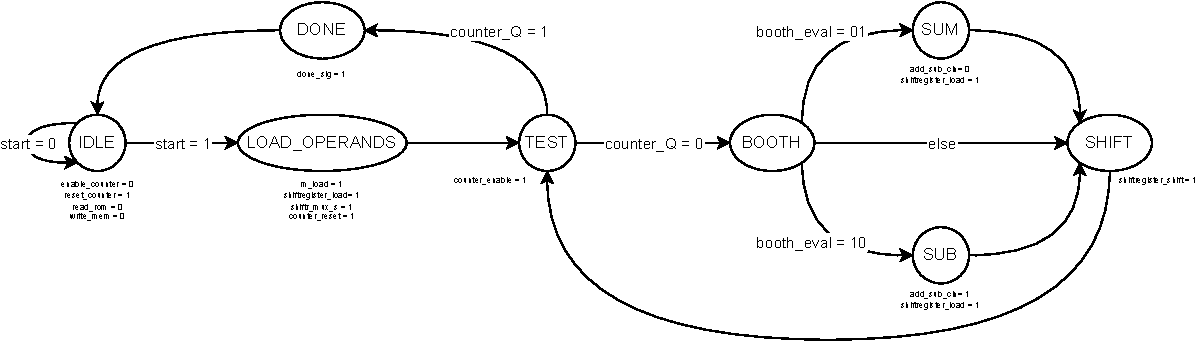
\includegraphics[width=\linewidth]{img/booth_multiplier.pdf}
    \caption{Automa del moltiplicatore di Booth}
    \label{fig:booth_multiplier}
\end{figure}

\begin{figure}[h]
    \centering
    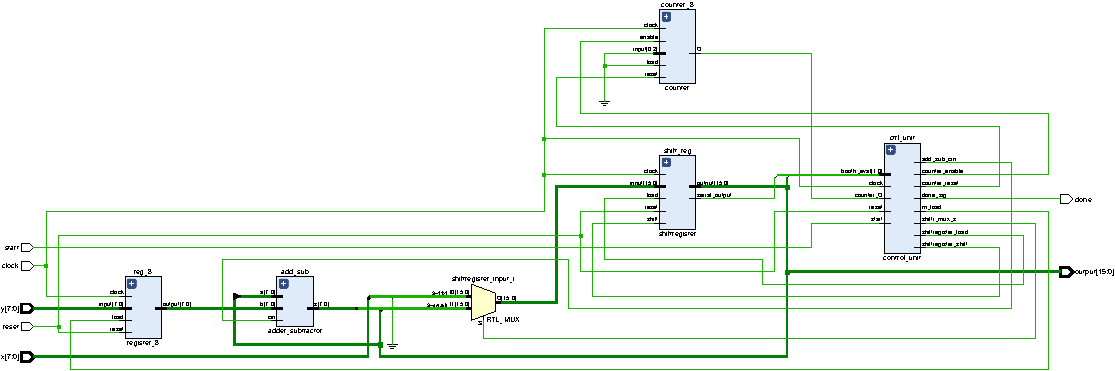
\includegraphics[width=\linewidth]{img/7_1_BOOTH_MULTIPLIER.pdf}
    \caption{Schema a blocchi del moltiplicatore di Booth}
    \label{fig:7_1_BOOTH_MULTIPLIER}
\end{figure}

\subsubsection{Implementazione}

\begin{code}
    \inputminted{vhdl}{vhdl/booth_multiplier.vhd}
    \caption{Implementazione del moltiplicatore di Booth}
    \label{cod:booth_multiplier}
\end{code}

\begin{code}
    \inputminted{vhdl}{vhdl/booth_multiplier_control_unit.vhd}
    \caption{Implementazione dell'unità di controllo}
    \label{cod:booth_multiplier_control_unit}
\end{code}

\paragraph{Funzionamento generale.}
L'algoritmo lavora esaminando gli ultimi due bit del moltiplicatore ($X$) e decide, in base a questi, se sommare, sottrarre o solo effettuare uno shift. Questo permette di ridurre il numero di operazioni necessarie per la moltiplicazione.

Per ogni ciclo dell'algoritmo, si osservano gli ultimi due bit del moltiplicatore ($X_j$ e $X_{j-1}$):

\begin{table}[h]
    \centering
    \begin{tabular}{|p{2cm}|p{10cm}|}
        \hline
        $X_j$$X_{j-1}$ & \textbf{Operazione} \\ \hline
        00/11 & Non viene effettuata né la somma né la sottrazione, ma solo lo shift. \\ \hline
        01 & Y viene aggiunto al prodotto parziale corrente. \\ \hline
        10 & Y viene sottratto al prodotto parziale corrente. \\ \hline
    \end{tabular}
\end{table}

Dopo l'operazione, il valore viene shiftato a destra e il processo continua per 8 iterazioni.

\paragraph{Struttura del codice.}
Il codice, essendo l'architettura \texttt{structural}, è diviso in più componenti, ognuno dei quali ha una funzione specifica:

\begin{enumerate}
    \item \texttt{register\_8} [Codice sorgente \ref{cod:register_8}]: memorizza il moltiplicando \texttt{y} e il valore viene caricato quando \texttt{m\_load = `1'}.
    \item \texttt{adder\_subtractor} [Codice sorgente \ref{cod:adder_subtractor}]: somma o sottrae \texttt{b} (collegato al registro contenente il moltiplicando $Y$) al registro parziale del risultato (\texttt{a}) in base ai bit $X_j$ e $X_{j-1}$, con il carry-in (\texttt{cin}) che determina se deve essere eseguita una somma o sottrazione.
    \item \texttt{shiftregister} [Codice sorgente \ref{cod:shiftregister}]: contiene il valore combinato (\texttt{A} e \texttt{Q}) dove:
    \begin{itemize}
        \item \texttt{A} contiene parte alta del risultato parziale (accumulatore).
        \item \texttt{Q} contiene inizialmente il moltiplicatore $X$ e via via parte del risultato.
    \end{itemize}
    Esegue lo shift a destra dopo ogni ciclo per aggiornare i bit da analizzare.
    \item \texttt{counter} [Codice sorgente \ref{cod:counter_risingedge}]: tiene traccia del numero di iterazioni eseguite, fermandosi dopo 8 iterazioni (il segnale \texttt{done} viene attivato e il risultato (\texttt{output}) è pronto).
    \item \texttt{control\_unit} [Codice sorgente \ref{cod:booth_multiplier_control_unit}]: decide quale operazione eseguire (somma, sottrazione o shift), gestendo il flusso dell'algoritmo:
    \begin{itemize}
        \item Se \texttt{booth\_eval = ``10"}, il moltiplicatore viene sottratto.
        \item Se \texttt{booth\_eval = ``01"}, il moltiplicatore viene aggiunto.
        \item Se \texttt{booth\_eval = ``00"} o ``11", viene eseguito solo lo shift.
    \end{itemize}
    Controlla anche i segnali:
    \begin{itemize}
        \item \texttt{shiftregister\_shift}, che abilita lo shift.
        \item \texttt{shiftregister\_load}, che carica lo shift register con il moltiplicatore e con i prodotti parziali.
        \item \texttt{m\_load}, che carica il moltiplicando $Y$.
        \item \texttt{counter\_enable}, che abilita il contatore.
        \item \texttt{done\_sig}, che indica che la moltiplicazione è terminata.
    \end{itemize}
\end{enumerate}

\subsubsection{Simulazione}
Per effettuare la simulazione il primo passo da compiere è la stesura del testbench. Prima di discuterne, è stato riportato il seguente codice:

\begin{code}
    \inputminted{vhdl}{vhdl/booth_multiplier_tb.vhd}
    \caption{Testbench del moltiplicatore di Booth}
    \label{cod:booth_multiplier_tb}
\end{code}

Esso verifica il corretto funzionamento del moltiplicatore di Booth.

La prima operazione svolta è stata la dichiarazione di un’entity. Si può notare che il corpo dell’entity è vuoto, poiché il testbench non rappresenta un componente hardware da implementare, ma serve esclusivamente per la simulazione e la verifica del corretto funzionamento del sistema.

\paragraph{Struttura del testbench.} Il testbench è strutturato in questo modo:

\begin{enumerate}
    \item Dichiarazione del componente da testare (\texttt{booth\_multiplier}):
    \begin{itemize}
        \item \texttt{x} e \texttt{y}: operandi della moltiplicazione (8 bit).
        \item \texttt{output}: risultato della moltiplicazione (16 bit).
        \item \texttt{clock}, \texttt{reset}, \texttt{start}: controllano l'esecuzione dell'operazione.
        \item \texttt{done}: indica quando la moltiplicazione è completata.
    \end{itemize}
    \item Generazione del clock con un processo (\texttt{CLK\_process}):
    \begin{itemize}
        \item Si genera un segnale di clock con un periodo di \texttt{10 ns}, il quale tra `0' e `1' ogni \texttt{5 ns}, simulando il funzionamento di un clock hardware.
    \end{itemize}
    \item Simulazione degli stimoli di ingresso (\texttt{stim\_proc}), dove vengono assegnati valori ai segnali di ingresso (\texttt{x}, \texttt{y}) e si verifica se il risultato (\texttt{output}) è corretto.
    \begin{itemize}
        \item Invia semplicemente i segnali di ingresso (\texttt{x}, \texttt{y}) al moltiplicatore e verifica i risultati attesi.
    \end{itemize}
    \item Verifica dell'output con \texttt{assert}, per confrontare i risultati ottenuti con quelli attesi.
    \begin{itemize}
        \item Se il valore atteso e il valore ottenuto non coincidono, viene generato un errore (\texttt{failure}).
        \item In caso di overflow, viene segnalato un avviso (\texttt{warning}), senza bloccare la simulazione.
    \end{itemize}
\end{enumerate}

\begin{figure}[h]
    \centering
    Prima moltiplicazione: $15 \cdot 3 = 45$
    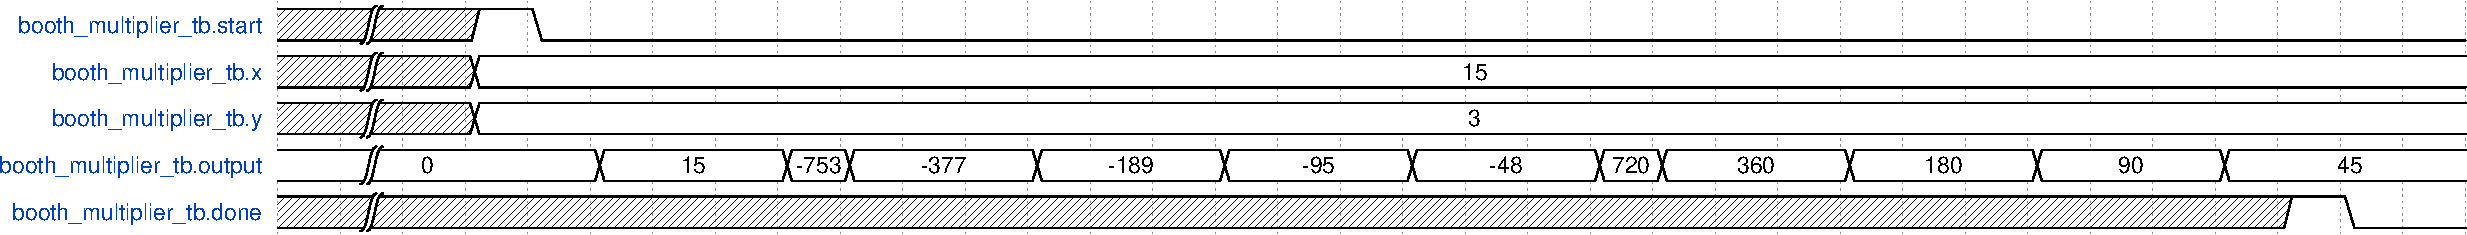
\includegraphics[width=\linewidth]{img/booth_multiplier_tb_1.pdf}
    \medskip

    Seconda moltiplicazione: $3 \cdot -5 = -15$
    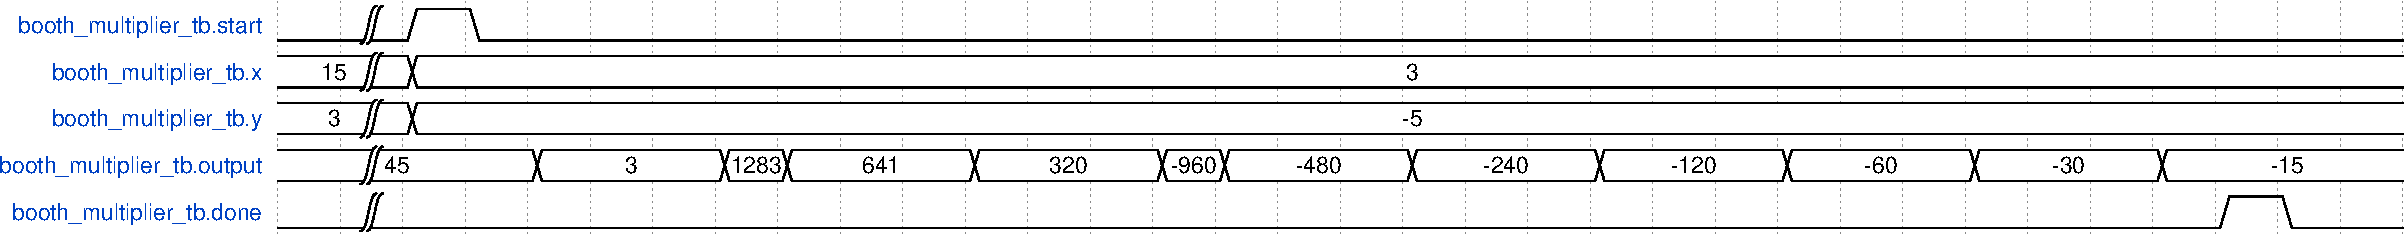
\includegraphics[width=\linewidth]{img/booth_multiplier_tb_2.pdf}
    \medskip

    Terza moltiplicazione: $-3 \cdot 3 = -9$
    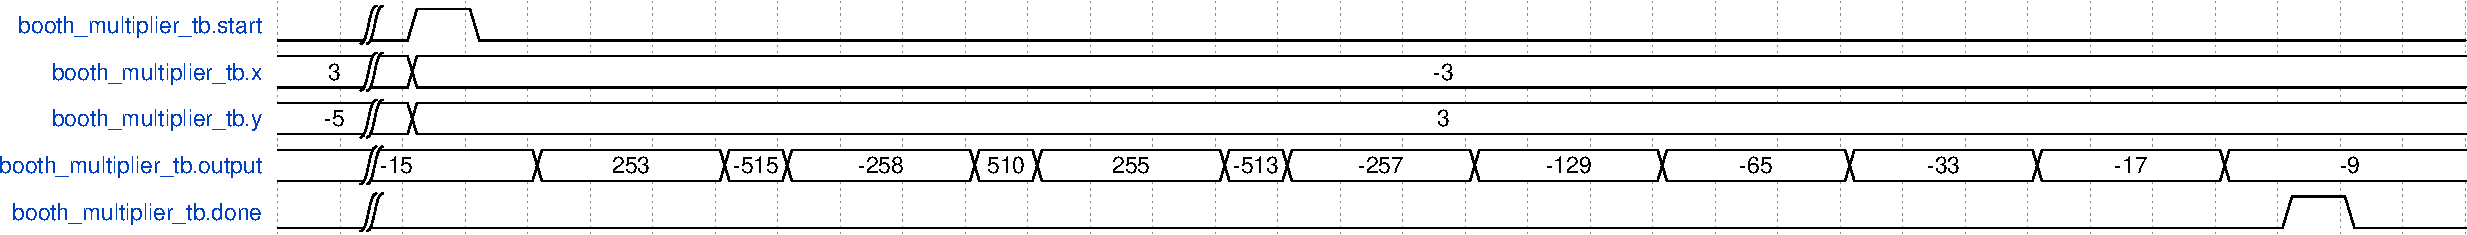
\includegraphics[width=\linewidth]{img/booth_multiplier_tb_3.pdf}
    \medskip

    Quarta moltiplicazione: $-3 \cdot -5 = 15$
    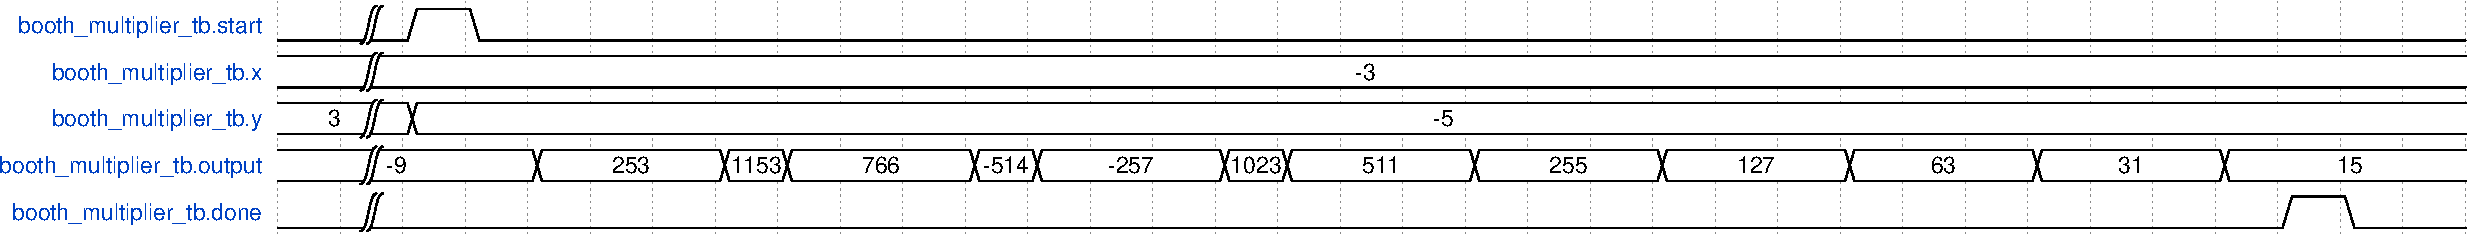
\includegraphics[width=\linewidth]{img/booth_multiplier_tb_4.pdf}
    \medskip

    Quinta moltiplicazione: $-128 \cdot -128 = 16384$ (overflow)
    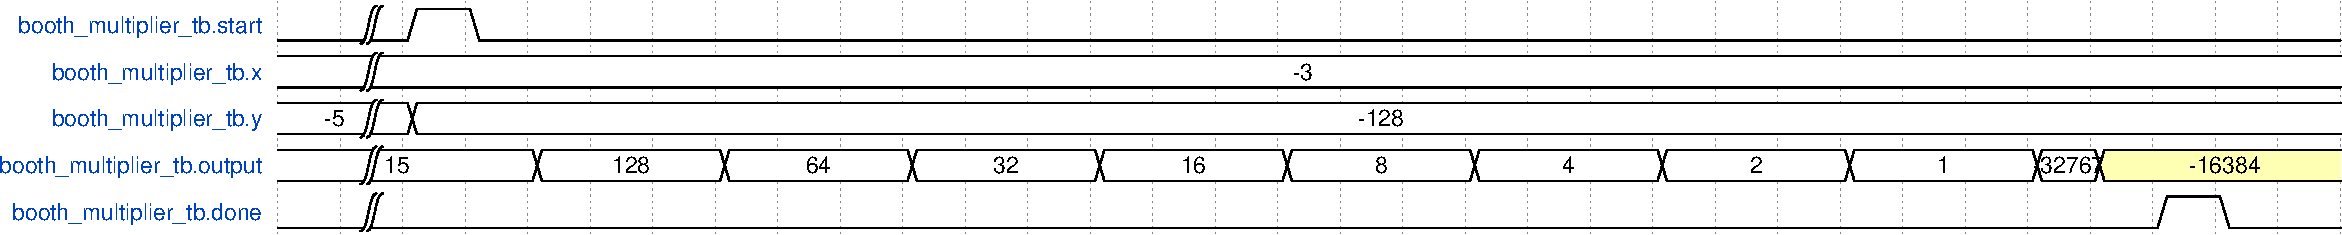
\includegraphics[width=\linewidth]{img/booth_multiplier_tb_5.pdf}
    \caption{Simulazione del moltiplicatore di Booth}
    \label{fig:booth_multiplier_tb}
\end{figure}

\subsection{Esercizio 7.2}
Si implementa un moltiplicatore di Booth su FPGA, permettendo l'interazione tramite switch, pulsanti e display a sette segmenti. L'obiettivo è moltiplicare due numeri binari forniti dagli switch, eseguire l'operazione quando il pulsante centrale viene premuto e mostrare il risultato sul display.

\begin{code}
    \inputminted{vhdl}{vhdl/booth_multiplier_onboard.vhd}
    \caption{Implementazione del moltiplicatore di Booth su board}
    \label{cod:booth_multiplier_onboard}
\end{code}

\begin{code}
    \inputminted{vhdl}{vhdl/booth_multiplier_seven_segments_display.vhd}
    \caption{Implementazione del display a 7 segmenti}
    \label{cod:booth_multiplier_seven_segments_display}
\end{code}

\begin{code}
    \inputminted{vhdl}{vhdl/booth_multiplier_cathodes_manager.vhd}
    \caption{Implementazione del gestore dei catodi}
    \label{cod:booth_multiplier_cathodes_manager}
\end{code}

\begin{code}
    \inputminted{vhdl}{vhdl/booth_multiplier_cathodes_input_manager.vhd}
    \caption{Implementazione del gestore degli input dei catodi}
    \label{cod:booth_multiplier_cathodes_input_manager}
\end{code}

\paragraph{Funzionamento generale.} Il sistema funziona nel seguente modo:

\begin{enumerate}
    \item Input degli operandi:
    \begin{itemize}
        \item Gli 8 switch di sinistra forniscono il moltiplicando ($Y$).
        \item Gli 8 switch di destra forniscono il moltiplicatore ($X$).
    \end{itemize}
    \item Avvio della moltiplicazione:
    \begin{itemize}
        \item Il pulsante centrale (BTNC) avvia il calcolo.
        \item Il pulsante superiore (BTNU) esegue il reset.
    \end{itemize}
    \item Elaborazione della moltiplicazione:
    \begin{itemize}
        \item Il moltiplicatore di Booth esegue l’operazione.
        \item I risultati parziali vengono mostrati in tempo reale sul display.
    \end{itemize}
    \item Indicazione del risultato finale:
    \begin{itemize}
        \item Quando il calcolo è completo, il primo LED di destra si accende.
        \item Il display a 7 segmenti mostra il risultato finale in decimale.
    \end{itemize}
\end{enumerate}

\paragraph{Struttura del codice.}
L’architettura è \texttt{structural} [Codice sorgente \ref{cod:booth_multiplier_onboard}], ovvero il sistema è composto da diversi moduli interconnessi:

\begin{enumerate}
    \item \texttt{booth\_multiplier} [Codice sorgente \ref{cod:booth_multiplier}]: componente che riceve il \texttt{clock}, \texttt{start}, operandi \texttt{x} e \texttt{y}, e produce il risultato (16 bit). Il segnale \texttt{done} indica quando il calcolo è terminato.
    \item \texttt{button\_debouncer} [Codice sorgente \ref{cod:button_debouncer}]: evita rimbalzi quando si preme il pulsante, stabilizzando il segnale \texttt{start}.
    \begin{itemize}
        \item \texttt{button}: ingresso dal pulsante.
        \item \texttt{button\_debounced}: segnale filtrato, privo di rimbalzi.
    \end{itemize}
    \item \texttt{seven\_segments\_display} [Codici sorgente \ref{cod:booth_multiplier_seven_segments_display}, \ref{cod:booth_multiplier_cathodes_manager}, \ref{cod:booth_multiplier_cathodes_input_manager}, \ref{cod:anodes_manager}]: mostra il risultato sul display a 7 segmenti.
    \begin{itemize}
        \item \texttt{input}: numero da visualizzare (16 bit).
        \item \texttt{enable}: seleziona quali cifre visualizzare.
        \item \texttt{anodes}, \texttt{cathodes}: controllano il display.
    \end{itemize}
\end{enumerate}

\paragraph{Collegamento dei Componenti.} I componenti vengono istanziati e collegati in maniera opportuna, ottenendo il sistema completo:

\begin{itemize}
    \item \texttt{start\_button}: semplicemente filtra il segnale \texttt{BTNC} e lo trasmette come \texttt{start} per avviare la moltiplicazione.
    \item \texttt{booth\_mult}: esegue la moltiplicazione e salva il risultato in \texttt{booth\_product} (16 bit). Il segnale \texttt{booth\_done} indica quando il calcolo è terminato.
    \item \texttt{ssd}: mostra semplicemente il risultato sul display a 7 segmenti.
    \item \texttt{led\_mgr}: il LED si accende quando \texttt{booth\_done = `1'}, indicando che il risultato finale è pronto.
\end{itemize}

Per poter utilizzare la board è stato necessario effettuare alcune modifiche al file dei constraints \texttt{Nexys A7-100T-Master.xdc}. In particolare, abbiamo dovuto aggiungere i seguenti vincoli:
\begin{itemize}
    \item Abilitare il clock a 100 MHz.
    \item Abilitare gli switch \texttt{SW0}--\texttt{SW15} per l’input.
    \item Abilitare i pulsanti \texttt{BTNC} per il segnale di \texttt{start}, \texttt{BTNU} per il reset.
    \item Abilitare il LED \texttt{LED0} per la visualizzazione del segnale \texttt{booth\_done}.
    \item Abilitare i catodi \texttt{CATHODES0}--\texttt{CATHODES7} e gli anodi \texttt{ANODES0}--\texttt{ANODES7} per l'utilizzo del display a sette segmenti.
\end{itemize}

\subsubsection{Timing Analysis}
Rispetto al design implementato al punto precedente, si può effettuare un'analisi temporale per verificare la tempificazione dei segnali.

Il sistema è stato implementato e risulta funzionante sulla board Nexys A7-100T. Attraverso il file dei constraints viene importato nel design il board clock a 100 MHz generato dall'oscillatore presente sulla board attraverso il pin \texttt{E3}. Questo segnale viene utilizzato per definire un \texttt{primary clock} con periodo di \texttt{10 ns} e duty cycle del 50\%.

Il progetto non prevede specifici vincoli riguardo il posizionamento dei componenti all'interno della FPGA, quindi il tool di sintesi è libero di posizionarli in maniera ottimale, ad esempio nella stessa clock region. Non sono stati impostati ulteriori vincoli.

Sono state eseguite sintesi ed implementazione del design, in particolare le fasi di ottimizzazione del design quali \texttt{opt\_design}, \texttt{place\_design} e \texttt{route\_design}. Il tool esegue poi un'analisi Min/Max per determinare i ritardi tra i clock di origine e desitinazione. Senza ulteriori accorgimenti, i dati temporali sono quelli in [Tabella \ref{tab:timing_analysis_10ns}].

\begin{table}[h!]
    \centering \scriptsize
    \begin{tabular}{p{4.8cm}p{4.8cm}p{4.8cm}}
        \hline
        \textbf{Setup} & \textbf{Hold} & \textbf{Pulse} \\
        Worst Negative Slack: \hfill 4.934 ns &
        Worst Hold Slack: \hfill 0.113 ns &
        Worst Pulse with Slack: \hfill 4.500 ns \\
        Total Negative Slack: \hfill 0.000 ns &
        Total Hold Slack: \hfill 0.000 ns &
        Total Pulse with Slack: \hfill 0.000 ns \\
        Number of Failing Endpoints: \hfill 0 &
        Number of Failing Endpoints: \hfill 0 &
        Number of Failing Endpoints: \hfill 0 \\
        Total Number of Endpoints: \hfill 189 &
        Total Number of Endpoints: \hfill 189 &
        Total Number of Endpoints: \hfill 111 \\
        \hline
    \end{tabular}
    \caption{Design Timing Summary con periodo di clock di 10 ns, duty cycle del 50\%}
    \label{tab:timing_analysis_10ns}
\end{table}

Il Worst Negative Slack è positivo, indicando che il design rispetta i vincoli temporali imposti. In base a quanto ottenuto, possiamo ottenere una stima grossolana del periodo di clock minimo per garantire il corretto funzionamento del sistema:

\begin{align*}
    T_{min} = T_{clk} - WNS = 10 ns - 4.934 ns = 5.066 ns \\
    F_{max} = \frac{1}{T_{clk} - WNS} = \frac{1}{10 ns - 4.934 ns} = 197 MHz
\end{align*}

Tuttavia, essendo i processi di \texttt{route\_design} e \texttt{place\_design} molto complessi e non compeltamente deterministici, non è detto che tali stime corrispondano al valore reale, nonostante ci consentano di avere un'idea generale dei limiti del sistema.

Per ottenere informazioni più precise, si procede con ulteriori test diminuendo il periodo di clock fino a raggiungere il limite di funzionamento del sistema. È importante tenere a mente che la frequenza ed il periodo di clock sono anche parametri in ingresso al sistema, per il corretto funzionamento del \texttt{button\_debouncer} e del \texttt{seven\_segments\_display}, di conseguenza al variare della frequenza del \texttt{primary\_clock} nel file dei constraints vanno modificati anche tali parametri all'interno del top module [Codice sorgente \ref{cod:booth_multiplier_onboard}]..

\begin{table}[h!]
    \centering \scriptsize
    \begin{tabular}{p{4.8cm}p{4.8cm}p{4.8cm}}
        \hline
        \textbf{Setup} & \textbf{Hold} & \textbf{Pulse} \\
        Worst Negative Slack: \hfill 0.639 ns &
        Worst Hold Slack: \hfill 0.187 ns &
        Worst Pulse with Slack: \hfill 2.000 ns \\
        Total Negative Slack: \hfill 0.000 ns &
        Total Hold Slack: \hfill 0.000 ns &
        Total Pulse with Slack: \hfill 0.000 ns \\
        Number of Failing Endpoints: \hfill 0 &
        Number of Failing Endpoints: \hfill 0 &
        Number of Failing Endpoints: \hfill 0 \\
        Total Number of Endpoints: \hfill 189 &
        Total Number of Endpoints: \hfill 189 &
        Total Number of Endpoints: \hfill 111 \\
        \hline
    \end{tabular}
    \caption{Design Timing Summary con periodo di clock di 5 ns, duty cycle del 50\%}
    \label{tab:timing_analysis_5ns}
\end{table}

Si nota in [Tabella \ref{tab:timing_analysis_5ns}] che con un periodo di 5 ns il Worst Negative Slack continua ad essere positivo e ben sopra la previsione precedente; questo poiché il tool di sintesi ha ottimizzato il design in maniera più efficiente, utilizzando path differenti e distribuendo diversamente i componenti nelle slice. Si può quindi provare a ridurre ulteriormente il periodo di clock:

\begin{table}[h!]
    \centering \scriptsize
    \begin{tabular}{p{4.8cm}p{4.8cm}p{4.8cm}}
        \hline
        \textbf{Setup} & \textbf{Hold} & \textbf{Pulse} \\
        Worst Negative Slack: \hfill 0.272 ns &
        Worst Hold Slack: \hfill 0.089 ns &
        Worst Pulse with Slack: \hfill 1.500 ns \\
        Total Negative Slack: \hfill 0.000 ns &
        Total Hold Slack: \hfill 0.000 ns &
        Total Pulse with Slack: \hfill 0.000 ns \\
        Number of Failing Endpoints: \hfill 0 &
        Number of Failing Endpoints: \hfill 0 &
        Number of Failing Endpoints: \hfill 0 \\
        Total Number of Endpoints: \hfill 190 &
        Total Number of Endpoints: \hfill 190 &
        Total Number of Endpoints: \hfill 112 \\
        \hline
    \end{tabular}
    \caption{Design Timing Summary con periodo di clock di 4 ns, duty cycle del 50\%}
    \label{tab:timing_analysis_4ns}
\end{table}

\begin{table}[h!]
    \centering \scriptsize
    \begin{tabular}{p{4.8cm}p{4.8cm}p{4.8cm}}
        \hline
        \textbf{Setup} & \textbf{Hold} & \textbf{Pulse} \\
        Worst Negative Slack: \hfill -0.775 ns &
        Worst Hold Slack: \hfill 0.195 ns &
        Worst Pulse with Slack: \hfill 0.845 ns \\
        Total Negative Slack: \hfill -23.750 ns &
        Total Hold Slack: \hfill 0.000 ns &
        Total Pulse with Slack: \hfill 0.000 ns \\
        Number of Failing Endpoints: \hfill 70 &
        Number of Failing Endpoints: \hfill 0 &
        Number of Failing Endpoints: \hfill 0 \\
        Total Number of Endpoints: \hfill 195 &
        Total Number of Endpoints: \hfill 195 &
        Total Number of Endpoints: \hfill 113 \\
        \hline
    \end{tabular}
    \caption{Design Timing Summary con periodo di clock di 3 ns, duty cycle del 50\%}
    \label{tab:timing_analysis_3ns}
\end{table}

Alla riduzione del periodo di clock a 3 ns, il Worst Negative Slack diventa negativo, indicando che il design non rispetta i vincoli temporali imposti. Questo comporta che il sistema non funzionerà correttamente, in quanto il clock non è in grado di distribuirsi in maniera corretta ai vari componenti. Si può quindi affermare che il periodo di clock minimo per garantire il corretto funzionamento del sistema è compreso tra 3 ns e 4 ns, ed una più precisa stima è:

\begin{align*}
    T_{min} = T_{clk} - WNS = 4 ns - 0.272 ns = 3.728 ns \\
    F_{max} = \frac{1}{T_{clk} - WNS} = \frac{1}{10 ns - 4.934 ns} = 268 MHz
\end{align*}

Dall'analisi del report Intra-Clock Paths si evince che il path critico è quello relativo al \texttt{button\_debouncer}, in particolare al bit meno significativi del registro associato alla variabile \texttt{count} dello stesso. Infatti, per il corretto funzionamento del sistema è necessario che essi si aggiornino ad una frequenza pari a quella del clock, tuttavia la propagazione del segnale non è sufficientemente veloce per garantire ciò.